% 2021 上海春季卷第 17 题；按固定副本第 2 页重绘可见拓扑与线型，坐标仅作投影示意。
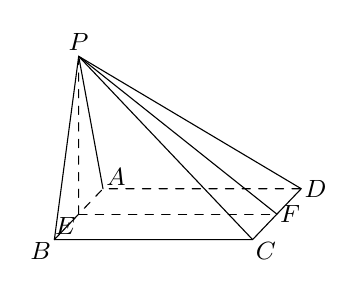
\begin{tikzpicture}[scale=.95,line cap=round,line join=round,font=\small]
  \coordinate (A) at (.65,.68);
  \coordinate (B) at (0,0);
  \coordinate (C) at (2.65,0);
  \coordinate (D) at (3.30,.68);
  \coordinate (E) at (.325,.34);
  \coordinate (F) at (2.975,.34);
  \coordinate (P) at (.325,2.45);

  \draw[dashed] (P) -- (E) -- (A) -- (D);
  \draw[dashed] (E) -- (F);
  \draw (P) -- (A);
  \draw (P) -- (B) -- (E);
  \draw (P) -- (D);
  \draw (P) -- (C);
  \draw (P) -- (F);
  \draw (B) -- (C) -- (F) -- (D);

  \node[above,inner sep=2pt] at (P) {$P$};
  \node[above right,inner sep=1pt] at (A) {$A$};
  \node[below left,inner sep=1pt] at (B) {$B$};
  \node[below right,inner sep=1pt] at (C) {$C$};
  \node[right,inner sep=1pt] at (D) {$D$};
  \node[below left,inner sep=1pt] at (E) {$E$};
  \node[right,inner sep=1pt] at (F) {$F$};
\end{tikzpicture}
